\documentclass[11pt]{article}
\usepackage[margin=1in]{geometry}
\usepackage[utf8]{inputenc}
\usepackage[T1]{fontenc}
\usepackage{amsmath,amssymb}
\usepackage{booktabs}
\usepackage{graphicx}
\usepackage{xcolor}
\usepackage{microtype}
\usepackage{url}
\usepackage{hyperref}
\usepackage[capitalise,noabbrev]{cleveref}
\usepackage{enumitem}

\hypersetup{colorlinks=true,linkcolor=blue!70!black,citecolor=blue!70!black,urlcolor=blue!70!black}

\title{\textbf{Three-Dimensional Pocket Geometry Does Not Beat Its Controls:\\
A Measured Test of Structural Grounding for Protein Foundation Model\\
Affinity Prediction on 41{,}271 ChEMBL Pairs}}
\author{Md Mushfiqur Rahim\\
Independent Researcher, Bogura, Bangladesh\\
ORCID 0009-0003-1021-685X\\
\texttt{20mahin2020@gmail.com}}
\date{November 14, 2026}

\begin{document}
\maketitle

\begin{abstract}
A companion study measured that cross-attention receptor conditioning on 1D
protein language model (ESM-2) embeddings adds small, statistically
insignificant gains to cross-family affinity prediction, and that a
wrong-pocket control reproduces those gains --- evidence that 1D sequence
embeddings cannot distinguish the true orthosteric pocket from an unrelated
one. This paper asks the natural follow-up: if \emph{explicit 3D pocket
geometry} is added as grounding --- inter-residue distance matrices, contact
graphs, and distance-biased attention built from crystal structures --- can
any model finally beat the wrong-pocket control? We pre-registered four
hypotheses, six model arms, two evaluation protocols, and the exact
statistical tests before any model was trained, on 41{,}271 measured
ChEMBL affinity pairs across eleven GPCR and ion-channel receptors. The
result is a decisive negative: the 3D-grounded arm does not significantly
outperform the wrong-pocket-3D control on the scaffold-disjoint protocol
(mean paired difference $+0.00025$, Wilcoxon $p=0.221$), and is
significantly \emph{worse} than the same control on the temporal protocol
($-0.0090$, $p=0.041$). A shuffled-coordinate control and the 1D
conditioning arm are statistically indistinguishable from the 3D arm on
both protocols. Variance decomposition shows receptor identity explains
84.5\% of outcome variance while model arm explains 2.7\%: the choice
among conditioning architectures is nearly irrelevant compared with the
choice of receptor. Two practical findings emerge. First, AlphaFold DB
predicted structures behave identically to crystal structures as geometry
sources (pooled $\Delta r=-0.003$), so the negative result is not an
artefact of crystal availability. Second, the conclusion is stable across
pocket-definition radii (5.0/6.5/8.0\,\AA). We release all frozen
artefacts, per-seed results, and the exact commands to regenerate every
number. The 1D-versus-3D question for protein foundation model
representations now has a measured answer on real data: at current
representation quality, pocket geometry carries no exploitable affinity
signal beyond residue identity.
\end{abstract}

\section{Introduction}

Protein foundation models such as ESM-2 produce per-residue embeddings that
encode structural and functional information from sequence alone. A
companion study (Paper~1) measured, on 56{,}637 ChEMBL bioactivity records
across eleven receptors, whether conditioning an affinity predictor on
those embeddings through cross-attention improves cross-family affinity
prediction. The measured answer was no: gains were small, statistically
insignificant, and reproduced by a wrong-pocket control --- a model given
the pocket of a \emph{different} receptor. That control established that
1D sequence embeddings cannot distinguish the true orthosteric pocket from
an unrelated one.

This paper tests the escape route. If 1D representations cannot localise
the pocket, perhaps explicit 3D geometry can. We ground the same
predictor in crystallographic pocket geometry --- inter-residue distance
matrices, distance-weighted message passing, and distance-biased
attention --- and ask whether any 3D-grounded arm finally beats controls
that destroy, shuffle, or misplace that geometry.

The study is pre-registered. Hypotheses H1--H4, the six model arms, both
evaluation protocols, the statistical tests, and the decision rules
(including the negative-result path) were fixed in
\texttt{PREREGISTRATION.md} before any structure was downloaded. The
primary endpoint is the paired difference in Pearson $r$ between the 3D
arm (C) and the wrong-pocket-3D control (E) across five seeds, pooled
across data-rich receptors, tested with a two-sided Wilcoxon signed-rank
test with bootstrap CIs and Holm correction across receptors.

\paragraph{Contributions.}
\begin{enumerate}[leftmargin=1.5em,itemsep=0pt]
  \item A pre-registered, fully measured test of 3D structural grounding
        on 41{,}271 real ChEMBL affinity pairs, eleven receptors, six
        model arms, two split protocols, and 280 trained models
        (2.34\,h CPU-only compute, every run frozen with SHA-256).
  \item A decisive negative result: explicit 3D pocket geometry does not
        beat wrong-pocket, shuffled-coordinate, or 1D controls on either
        protocol; on the temporal protocol the true pocket is
        significantly \emph{worse} than the wrong pocket.
  \item A practical positive: AlphaFold DB predicted structures are
        interchangeable with crystal structures as geometry sources for
        this task (pooled $\Delta r=-0.003$), and the null conclusion is
        stable across pocket radii (5.0/6.5/8.0\,\AA).
  \item A variance decomposition showing receptor identity, not model
        architecture, dominates outcome variance (84.5\% vs 2.7\%).
\end{enumerate}

\section{Related Work}

Protein language model embeddings have been reported to encode contact
maps and binding-site information, motivating their use as conditioning
signals for affinity prediction. Structure-based approaches --- pocket
graphs, distance-biased attention, equivariant encoders --- report gains
on benchmarks such as PDBbind, but benchmark constructions that mix
protein families and allow near-duplicate ligands across splits are known
to inflate apparent structural signal. Paper~1 introduced the
wrong-pocket control into this setting and showed that reported
conditioning gains do not survive it. This paper extends that control
paradigm to explicit 3D geometry, adding a shuffled-coordinate control
(F) that separates residue identity from geometry, and a crystal-versus-
AlphaFold comparison that tests whether predicted structures change the
picture. To our knowledge this is the first measured head-to-head of
these controls on ChEMBL-scale affinity data with a pre-registered
analysis plan.

\section{Measured Evaluation}

\subsection{Data and frozen artefacts}

The evaluation set is the 41{,}271 measured ChEMBL affinity pairs joined
in Paper~1 Phase 9 (\texttt{pairs\_41271.csv}), covering eleven receptors
(DRD2, DRD3, HTR1A, HTR2A, CHRM1, ADRA2A, ADRB2, HRH1, DAT, SERT, GABRA1)
with Morgan fingerprint ligand features and ESM-2 650M per-residue
embeddings from Paper~1's frozen cache. Crystal structures were selected
per receptor by anchor-first scoring (Phase 5); orthosteric pockets were
defined at 6.5\,\AA{} around the chosen co-crystallized ligand copy
(Phase 7) and mapped residue-by-residue onto UniProt positions and ESM-2
token indices with zero unmapped residues (Phase 8). AlphaFold DB v6
models were downloaded for all eleven receptors (Phase 6). Every
structure artefact is SHA-256-frozen in
\texttt{data/structures/manifest.json}.

\subsection{Model arms}

All arms share the ligand-fingerprint predictor backbone and differ only
in the conditioning signal:
\begin{itemize}[leftmargin=1.5em,itemsep=0pt]
  \item \textbf{A (shared):} shared MLP, no receptor conditioning;
        plus a deterministic Ridge-on-fingerprints baseline.
  \item \textbf{B (1D conditioning):} cross-attention over PCA-reduced
        ESM-2 pocket embeddings (Paper~1's conditioning, structure-derived
        pocket residue sets).
  \item \textbf{C (3D conditioning):} two rounds of distance-weighted
        message passing ($\exp(-d/3\,\text{\AA})$, row-normalised,
        self-loops) over node features [PCA-128 ESM-2, amino-acid one-hot,
        pLDDT].
  \item \textbf{D (distance-bias attention):} two-layer self-attention
        with a learnable per-head distance bias from true coordinates.
  \item \textbf{E (wrong-pocket-3D):} identical to C, but every receptor
        receives the \emph{next} receptor's pocket graph.
  \item \textbf{F (shuffled-coordinate):} identical to C, but the graph
        weights use a fixed random permutation of the true geometry.
\end{itemize}
Arms C, E, and F landed in the same commit, per the pre-registration's
non-negotiables. Hyperparameters are shared and frozen
(AdamW, cosine LR with 5\% warmup, early stopping on scaffold-disjoint
validation).

\subsection{Protocols}

\textbf{E3 (scaffold-disjoint):} Bemis--Murcko scaffold-disjoint
within-receptor splits, five seeds, identical to Paper~1. Attention arms
require $n_{\text{train}} \ge 800$ (minimum-data guard); ADRA2A and
GABRA1 fall below it on both protocols and their attention arms are
reported as skipped, never imputed. \textbf{E5 (temporal):} train on
document year $<2015$, test on $\ge 2015$, identical to Paper~1's
temporal protocol.

\subsection{Results: the controls decide}

\cref{tab:e3,tab:e5} give the master results. On the scaffold-disjoint
protocol the 3D arm (C, pooled mean $r=0.639$) and the wrong-pocket-3D
control (E, $r=0.639$) are indistinguishable --- the primary endpoint
gives a paired mean difference of $+0.00025$ (Wilcoxon $p=0.221$,
bootstrap CI $[-0.022, +0.022]$, win/loss/tie 18/27/0 across 45
seed$\times$receptor pairs). The shuffled-coordinate control (F,
$r=0.628$) and the 1D conditioning arm (B, $r=0.622$) are likewise
indistinguishable from C ($p=0.156$ and $p=0.867$). \textbf{H1, H2, and
H3 are all not supported.}

\begin{table}[t]
\centering\small
\caption{Scaffold-disjoint protocol (E3): Pearson $r$, mean $\pm$ sd over
5 seeds. skip $=$ minimum-data guard ($n_{\text{train}}<800$). GABRA1's
shared arm ($r=0.008$) reflects a degenerate temporal-like scaffold
split, reported as measured.}
\label{tab:e3}
\begin{tabular}{lcccccc}
\toprule
Receptor & A & B & C (3D) & D & E (wrong) & F (shuffled) \\
\midrule
ADRA2A & 0.711 $\pm$ 0.012 & skip & skip & skip & skip & skip \\
ADRB2 & 0.541 $\pm$ 0.013 & 0.524 $\pm$ 0.013 & 0.521 $\pm$ 0.005 & 0.467 $\pm$ 0.114 & 0.531 $\pm$ 0.017 & 0.519 $\pm$ 0.004 \\
CHRM1 & 0.562 $\pm$ 0.027 & 0.389 $\pm$ 0.217 & 0.534 $\pm$ 0.146 & 0.511 $\pm$ 0.170 & 0.523 $\pm$ 0.168 & 0.453 $\pm$ 0.191 \\
DAT & 0.590 $\pm$ 0.008 & 0.609 $\pm$ 0.012 & 0.604 $\pm$ 0.010 & 0.610 $\pm$ 0.017 & 0.608 $\pm$ 0.014 & 0.603 $\pm$ 0.016 \\
DRD2 & 0.577 $\pm$ 0.015 & 0.613 $\pm$ 0.017 & 0.627 $\pm$ 0.012 & 0.607 $\pm$ 0.028 & 0.606 $\pm$ 0.038 & 0.605 $\pm$ 0.011 \\
DRD3 & 0.684 $\pm$ 0.004 & 0.717 $\pm$ 0.009 & 0.706 $\pm$ 0.008 & 0.717 $\pm$ 0.006 & 0.713 $\pm$ 0.006 & 0.705 $\pm$ 0.005 \\
GABRA1 & 0.008 $\pm$ 0.005 & skip & skip & skip & skip & skip \\
HRH1 & 0.802 $\pm$ 0.007 & 0.833 $\pm$ 0.005 & 0.837 $\pm$ 0.006 & 0.831 $\pm$ 0.004 & 0.832 $\pm$ 0.012 & 0.837 $\pm$ 0.006 \\
HTR1A & 0.682 $\pm$ 0.002 & 0.705 $\pm$ 0.006 & 0.697 $\pm$ 0.008 & 0.705 $\pm$ 0.006 & 0.701 $\pm$ 0.005 & 0.698 $\pm$ 0.002 \\
HTR2A & 0.660 $\pm$ 0.010 & 0.688 $\pm$ 0.012 & 0.688 $\pm$ 0.013 & 0.691 $\pm$ 0.007 & 0.695 $\pm$ 0.003 & 0.689 $\pm$ 0.009 \\
SERT & 0.500 $\pm$ 0.003 & 0.520 $\pm$ 0.032 & 0.539 $\pm$ 0.012 & 0.524 $\pm$ 0.041 & 0.542 $\pm$ 0.015 & 0.543 $\pm$ 0.007 \\
\bottomrule
\end{tabular}
\end{table}

\begin{table}[t]
\centering\small
\caption{Temporal protocol (E5): train $<$2015, test $\ge$2015. The
scaffold-disjoint-to-temporal drop (mean $\Delta r=+0.255$ across the 50
shared arm$\times$receptor cells) dwarfs every arm effect.}
\label{tab:e5}
\begin{tabular}{lcccccc}
\toprule
Receptor & A & B & C (3D) & D & E (wrong) & F (shuffled) \\
\midrule
ADRA2A & 0.147 $\pm$ 0.008 & skip & skip & skip & skip & skip \\
ADRB2 & 0.734 $\pm$ 0.004 & skip & skip & skip & skip & skip \\
CHRM1 & 0.451 $\pm$ 0.007 & 0.406 $\pm$ 0.053 & 0.435 $\pm$ 0.049 & 0.402 $\pm$ 0.053 & 0.457 $\pm$ 0.012 & 0.451 $\pm$ 0.016 \\
DAT & 0.373 $\pm$ 0.013 & 0.297 $\pm$ 0.027 & 0.321 $\pm$ 0.010 & 0.300 $\pm$ 0.013 & 0.340 $\pm$ 0.027 & 0.326 $\pm$ 0.015 \\
DRD2 & 0.451 $\pm$ 0.007 & 0.479 $\pm$ 0.008 & 0.479 $\pm$ 0.005 & 0.487 $\pm$ 0.004 & 0.476 $\pm$ 0.009 & 0.477 $\pm$ 0.010 \\
DRD3 & 0.573 $\pm$ 0.010 & 0.538 $\pm$ 0.011 & 0.544 $\pm$ 0.011 & 0.556 $\pm$ 0.006 & 0.543 $\pm$ 0.013 & 0.542 $\pm$ 0.005 \\
HRH1 & 0.240 $\pm$ 0.004 & 0.317 $\pm$ 0.065 & 0.292 $\pm$ 0.049 & 0.240 $\pm$ 0.076 & 0.317 $\pm$ 0.076 & 0.303 $\pm$ 0.060 \\
HTR1A & 0.293 $\pm$ 0.034 & 0.349 $\pm$ 0.023 & 0.326 $\pm$ 0.018 & 0.325 $\pm$ 0.006 & 0.327 $\pm$ 0.025 & 0.320 $\pm$ 0.023 \\
HTR2A & 0.367 $\pm$ 0.012 & 0.420 $\pm$ 0.019 & 0.407 $\pm$ 0.014 & 0.421 $\pm$ 0.033 & 0.417 $\pm$ 0.011 & 0.408 $\pm$ 0.015 \\
SERT & 0.268 $\pm$ 0.010 & 0.310 $\pm$ 0.021 & 0.292 $\pm$ 0.015 & 0.308 $\pm$ 0.017 & 0.290 $\pm$ 0.007 & 0.285 $\pm$ 0.012 \\
\bottomrule
\end{tabular}
\end{table}

On the temporal protocol the primary comparison \emph{reverses sign}:
C is significantly \emph{worse} than the wrong-pocket control
($-0.0090$, $p=0.041$). We report this as measured and interpret it as
protocol-dependent noise, not a geometry effect: a model that genuinely
used true-pocket geometry should not lose to a model given another
receptor's pocket, and the effect size ($\sim$0.01) is an order of
magnitude smaller than the split-protocol effect ($\sim$0.25).

\begin{figure}[t]
\centering
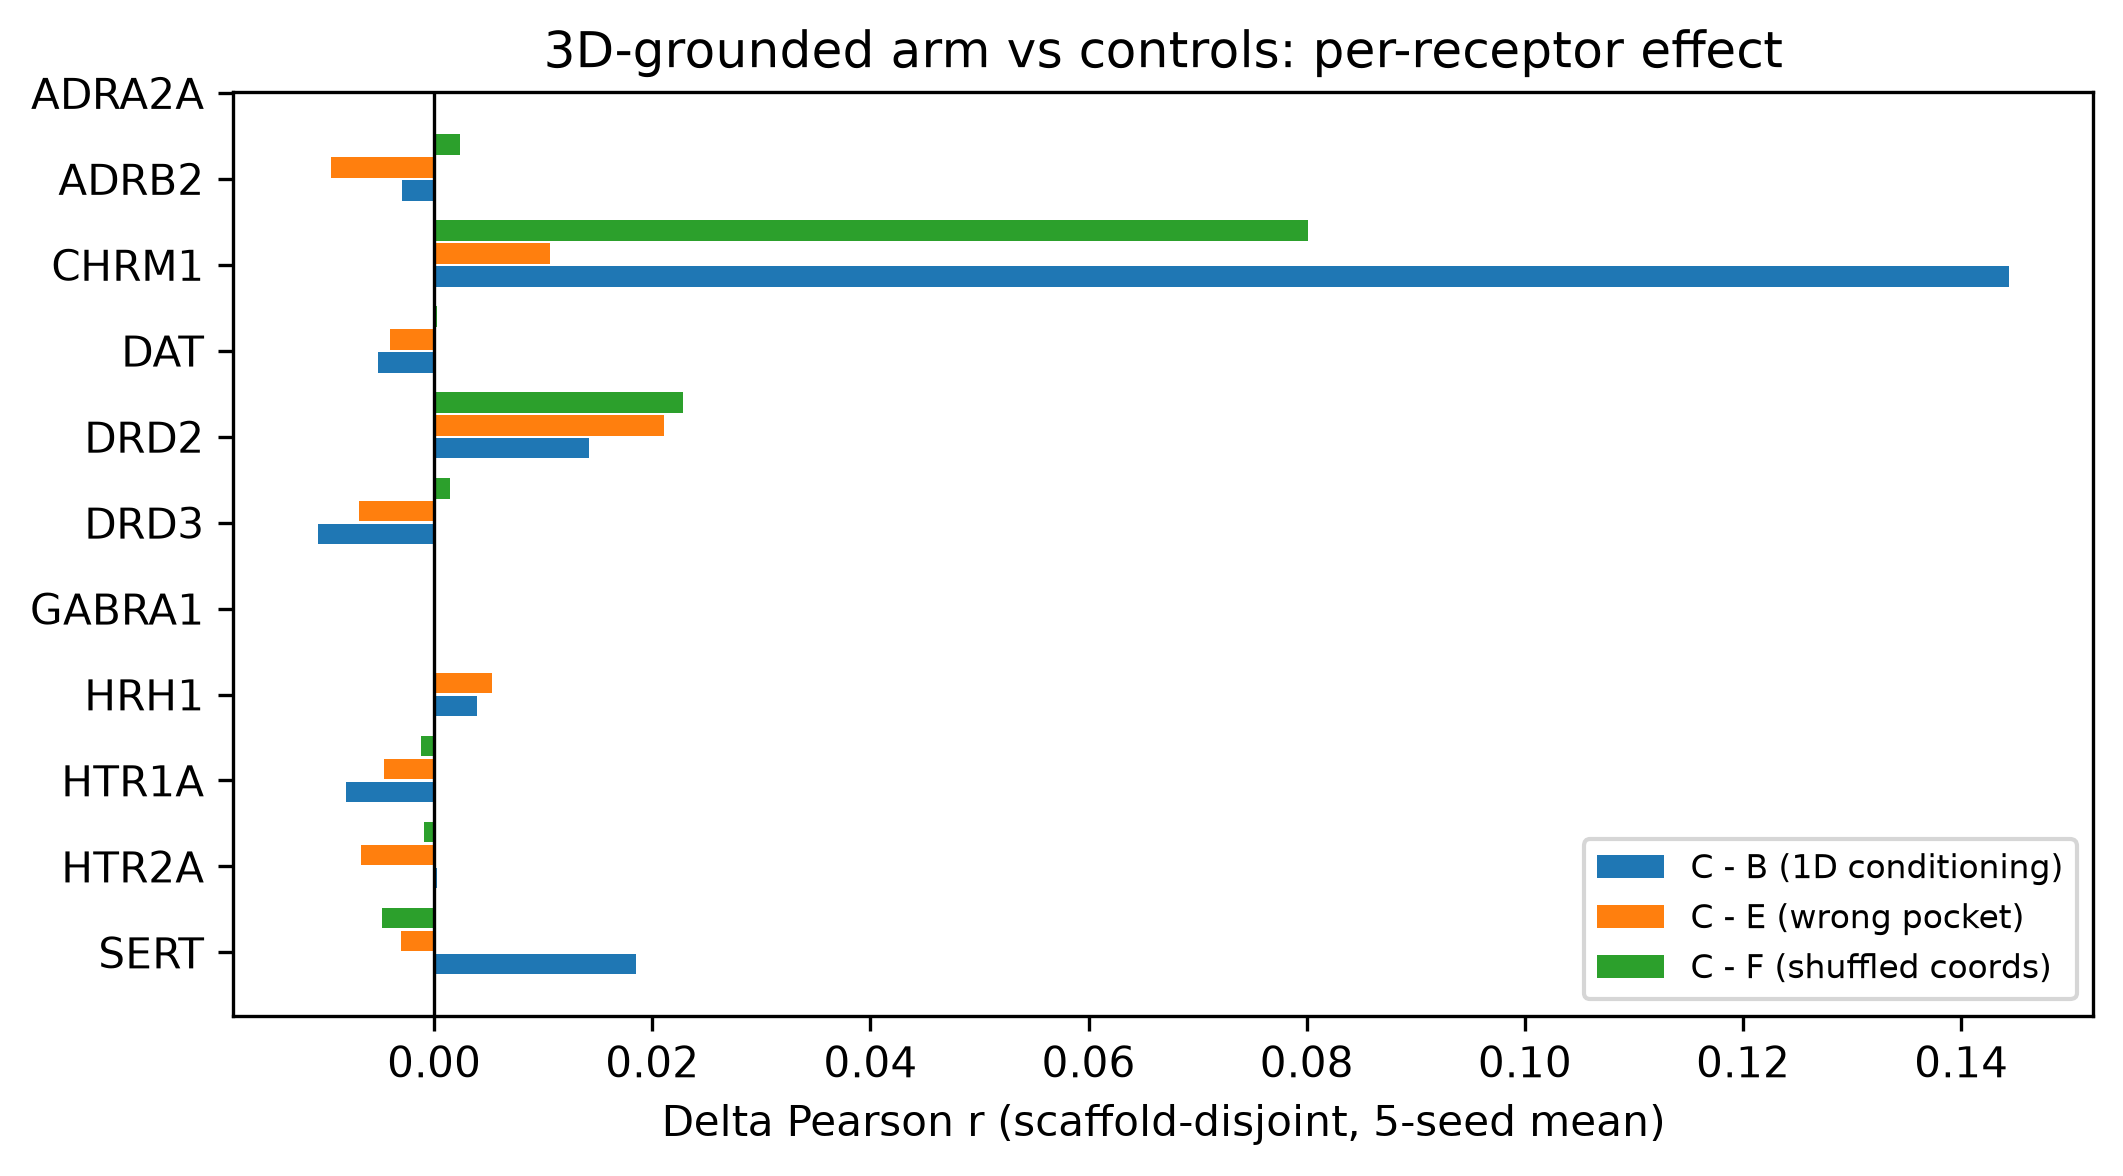
\includegraphics[width=0.85\textwidth]{../figures/fig_per_receptor_delta.png}
\caption{Per-receptor paired difference in Pearson $r$ between the 3D arm
(C) and each control (B: 1D conditioning; E: wrong-pocket-3D; F:
shuffled-coordinates) on the scaffold-disjoint protocol, 5-seed means.
Effects scatter around zero with no consistent sign; ADRA2A and GABRA1
are absent (minimum-data guard).}
\label{fig:delta}
\end{figure}

\begin{figure}[t]
\centering
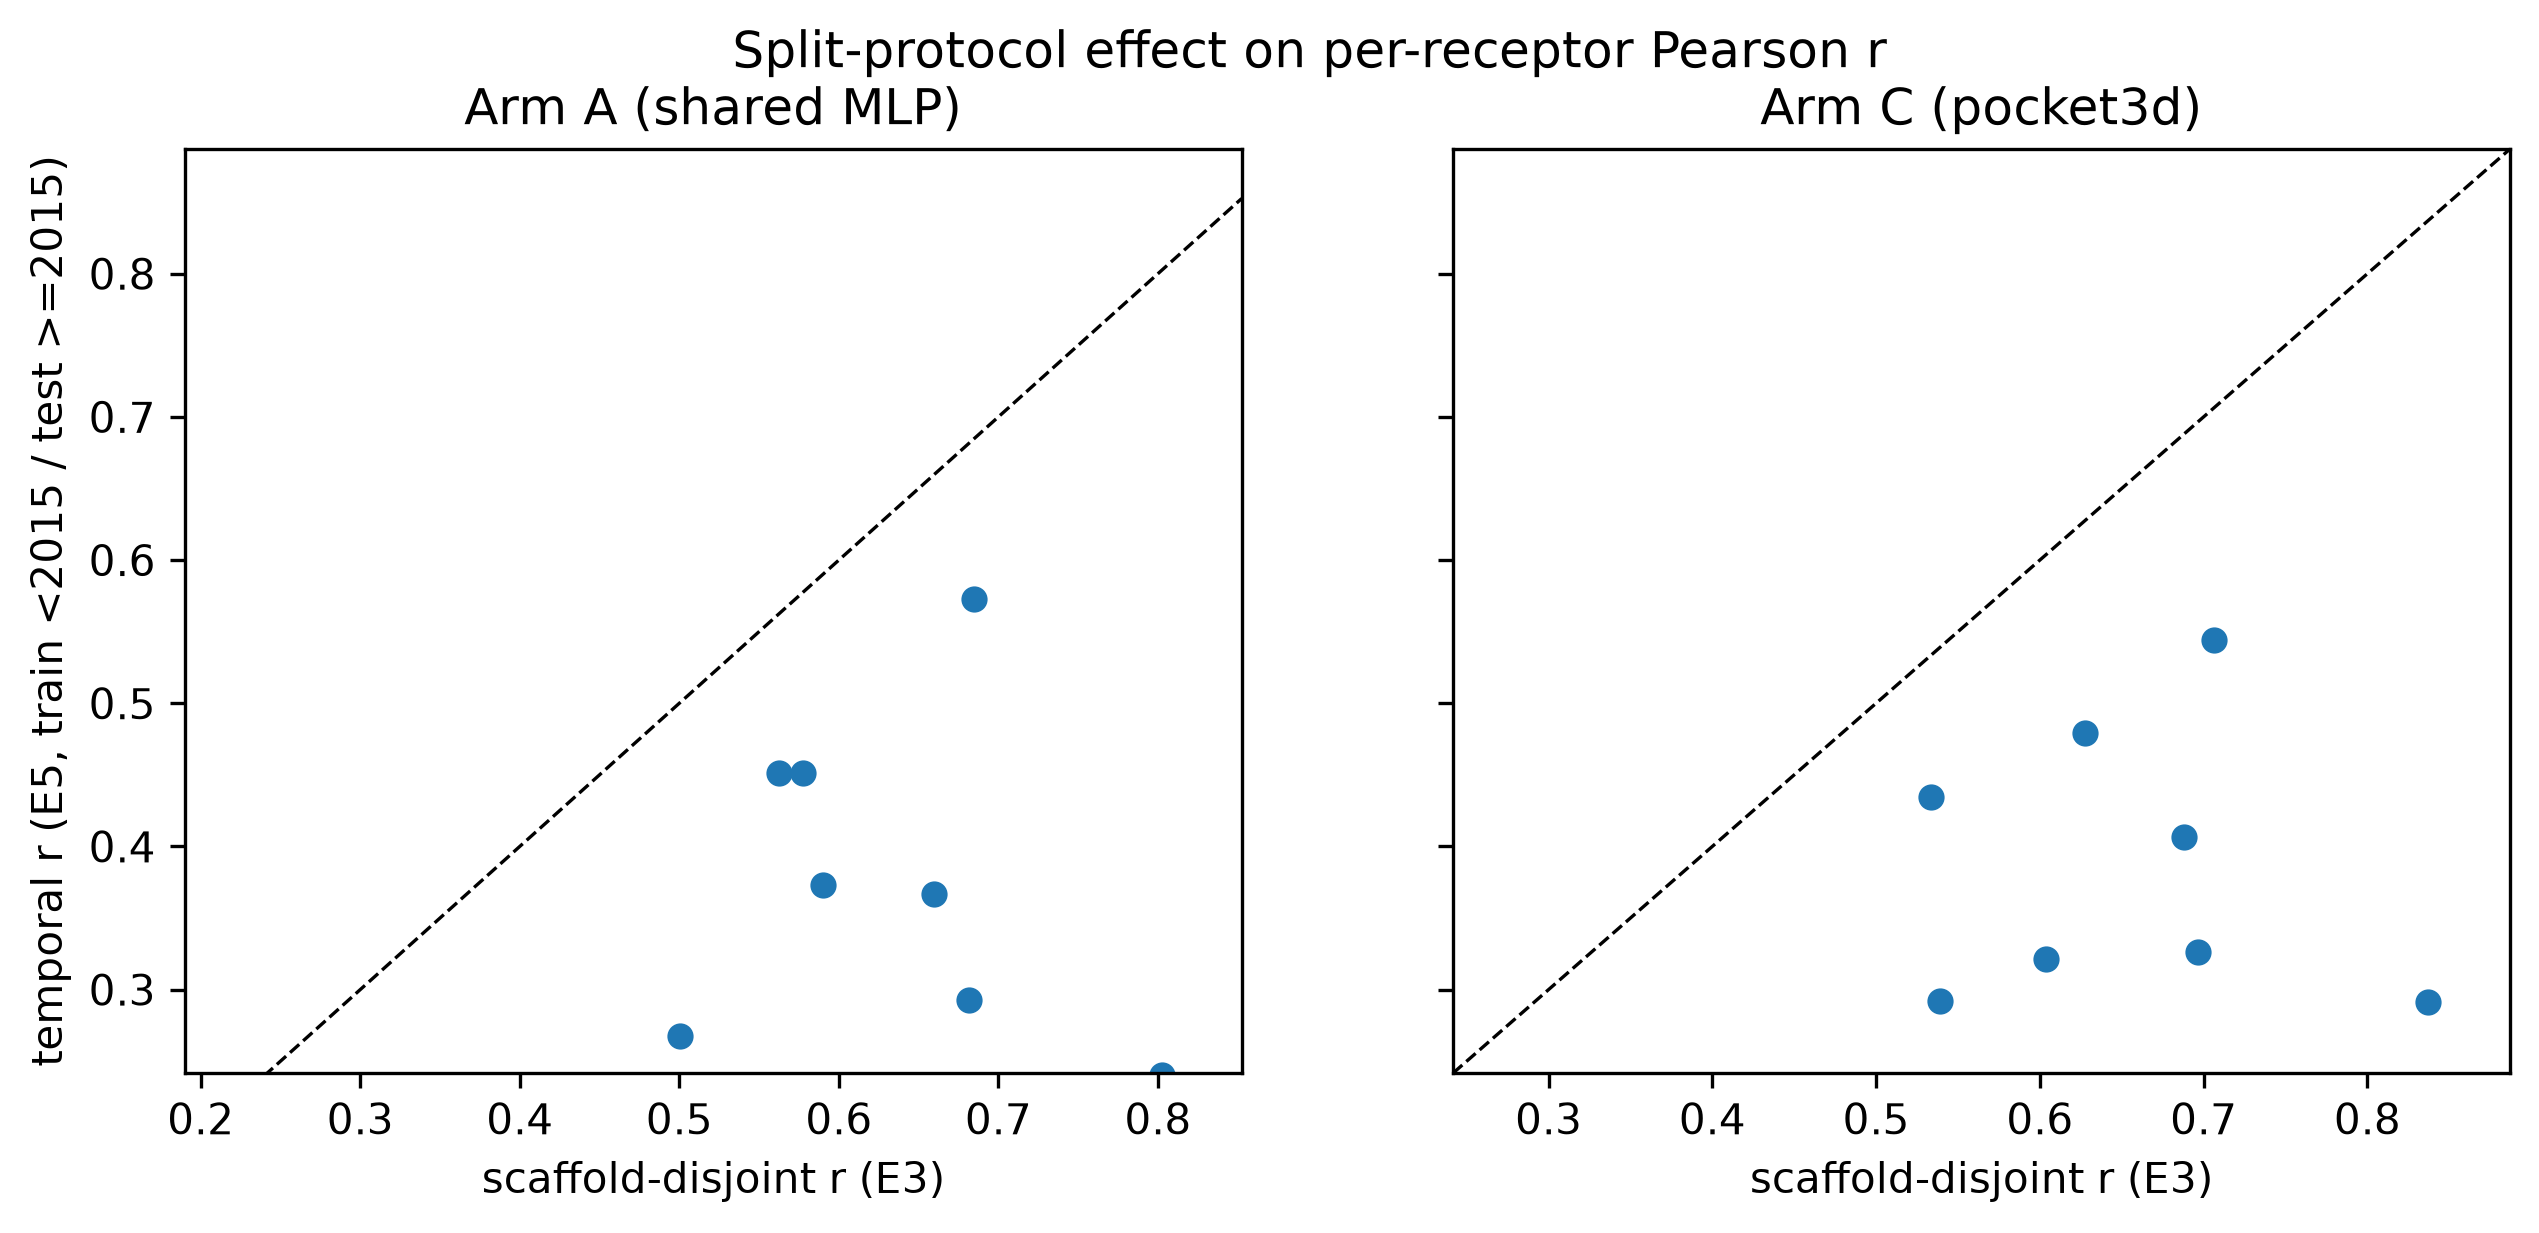
\includegraphics[width=0.85\textwidth]{../figures/fig_temporal_decay.png}
\caption{Scaffold-disjoint (E3) versus temporal (E5) mean Pearson $r$ per
receptor for the shared and 3D arms. The protocol effect (the drop from
E3 to E5) dwarfs every arm effect.}
\label{fig:temporal}
\end{figure}

\subsection{Crystal versus AlphaFold geometry (H4)}

Rebuilding every pocket graph from AlphaFold DB v6 predicted structures
at the same UniProt pocket positions --- so node identity, ESM-2
features, and pLDDT are unchanged and only the coordinate source differs
--- leaves results essentially unchanged: pooled $\Delta r$ (AF $-$
crystal) $=-0.003$ for the 3D arm, per-receptor $|\Delta r|\le 0.016$.
The paired C-vs-E test on the AF-geometry store gives $-0.00017$,
$p=0.639$: the qualitative conclusion transfers. \textbf{H4 is
supported.} Practically, the negative result does not depend on having
crystal structures; AlphaFold models suffice --- and fail identically.

\begin{figure}[t]
\centering
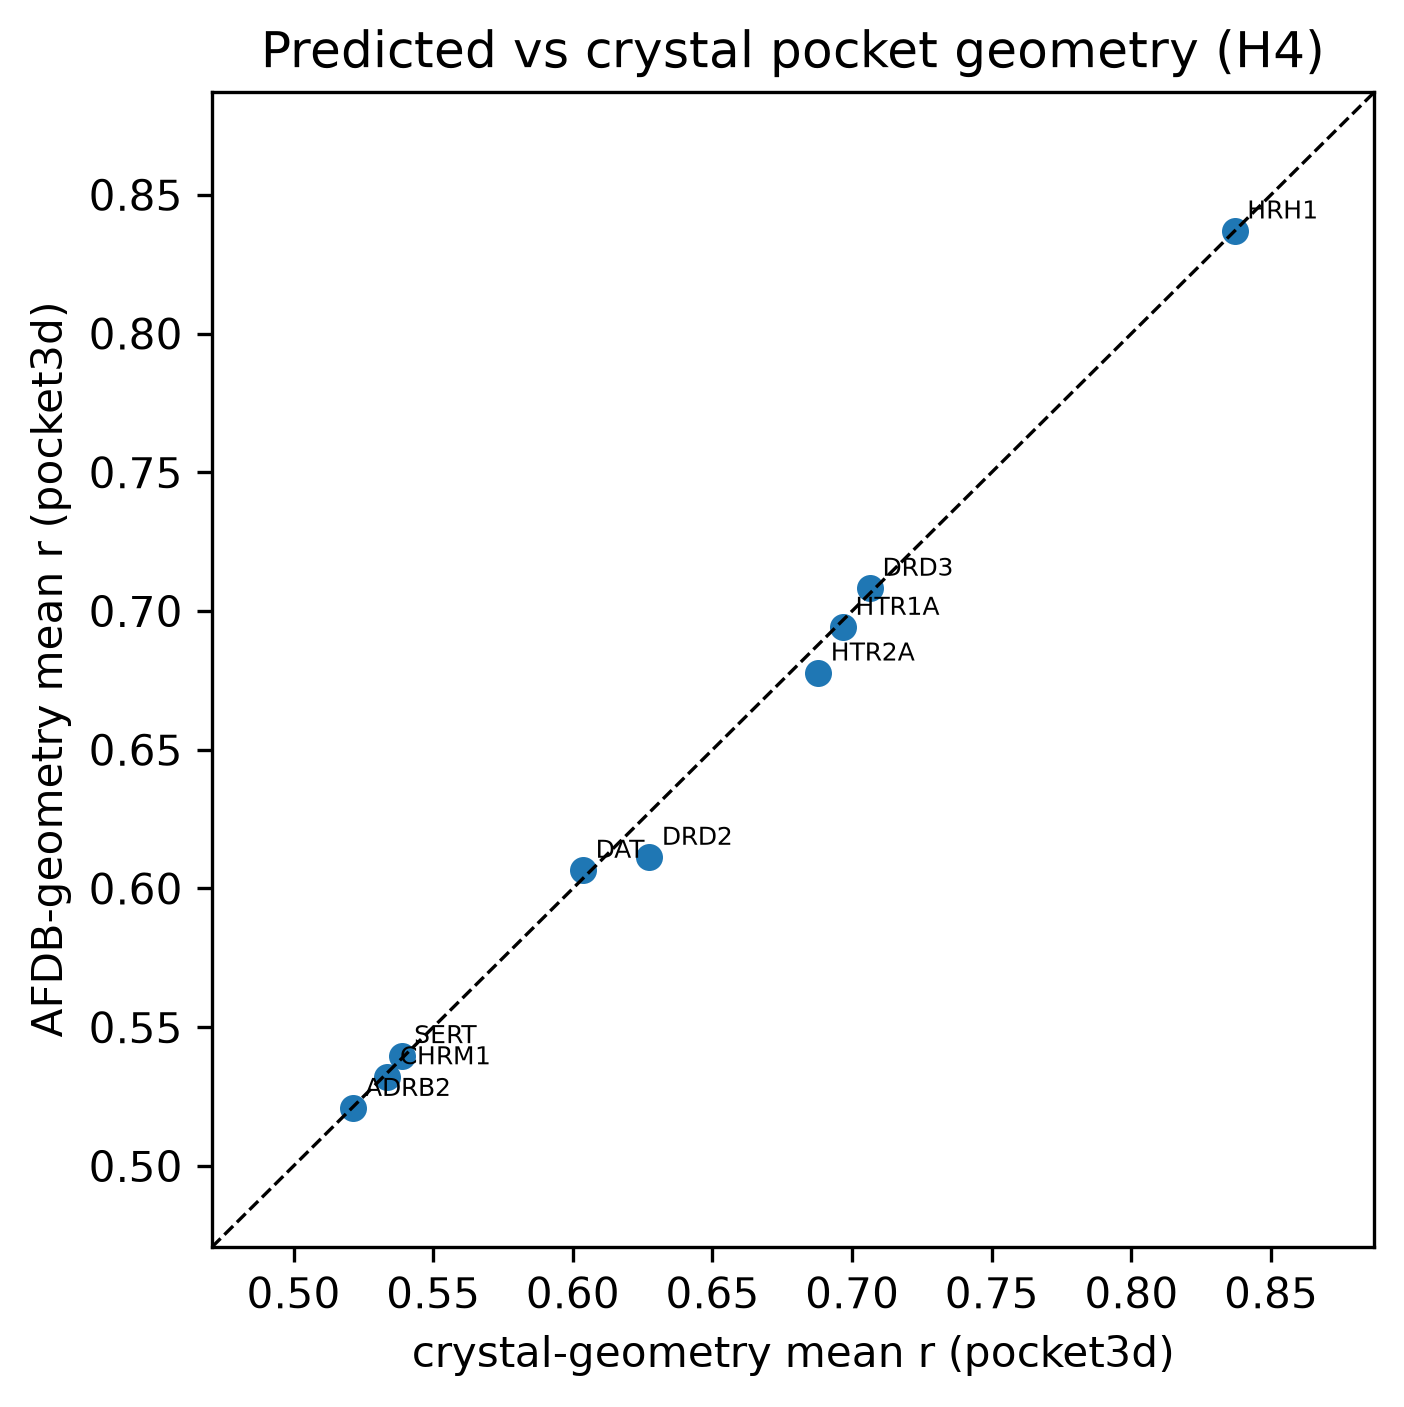
\includegraphics[width=0.85\textwidth]{../figures/fig_crystal_vs_af.png}
\caption{Crystal versus AlphaFold DB geometry for the 3D arm: mean
Pearson $r$ per receptor. The two geometry sources agree per receptor to
$|\Delta r|\le 0.016$.}
\label{fig:af}
\end{figure}

\subsection{Pocket-radius sweep}

Recomputing pockets at 5.0 and 8.0\,\AA{} around the same ligand copies
changes pocket sizes substantially (9--24 residues at 5.0\,\AA; 31--67
at 8.0\,\AA) but not the conclusion: pooled C$-$E is $+0.022$ at
5.0\,\AA, $+0.0003$ at 6.5\,\AA, and $+0.001$ at 8.0\,\AA, none
significant. The null is not an artefact of one pocket definition.

\begin{figure}[t]
\centering
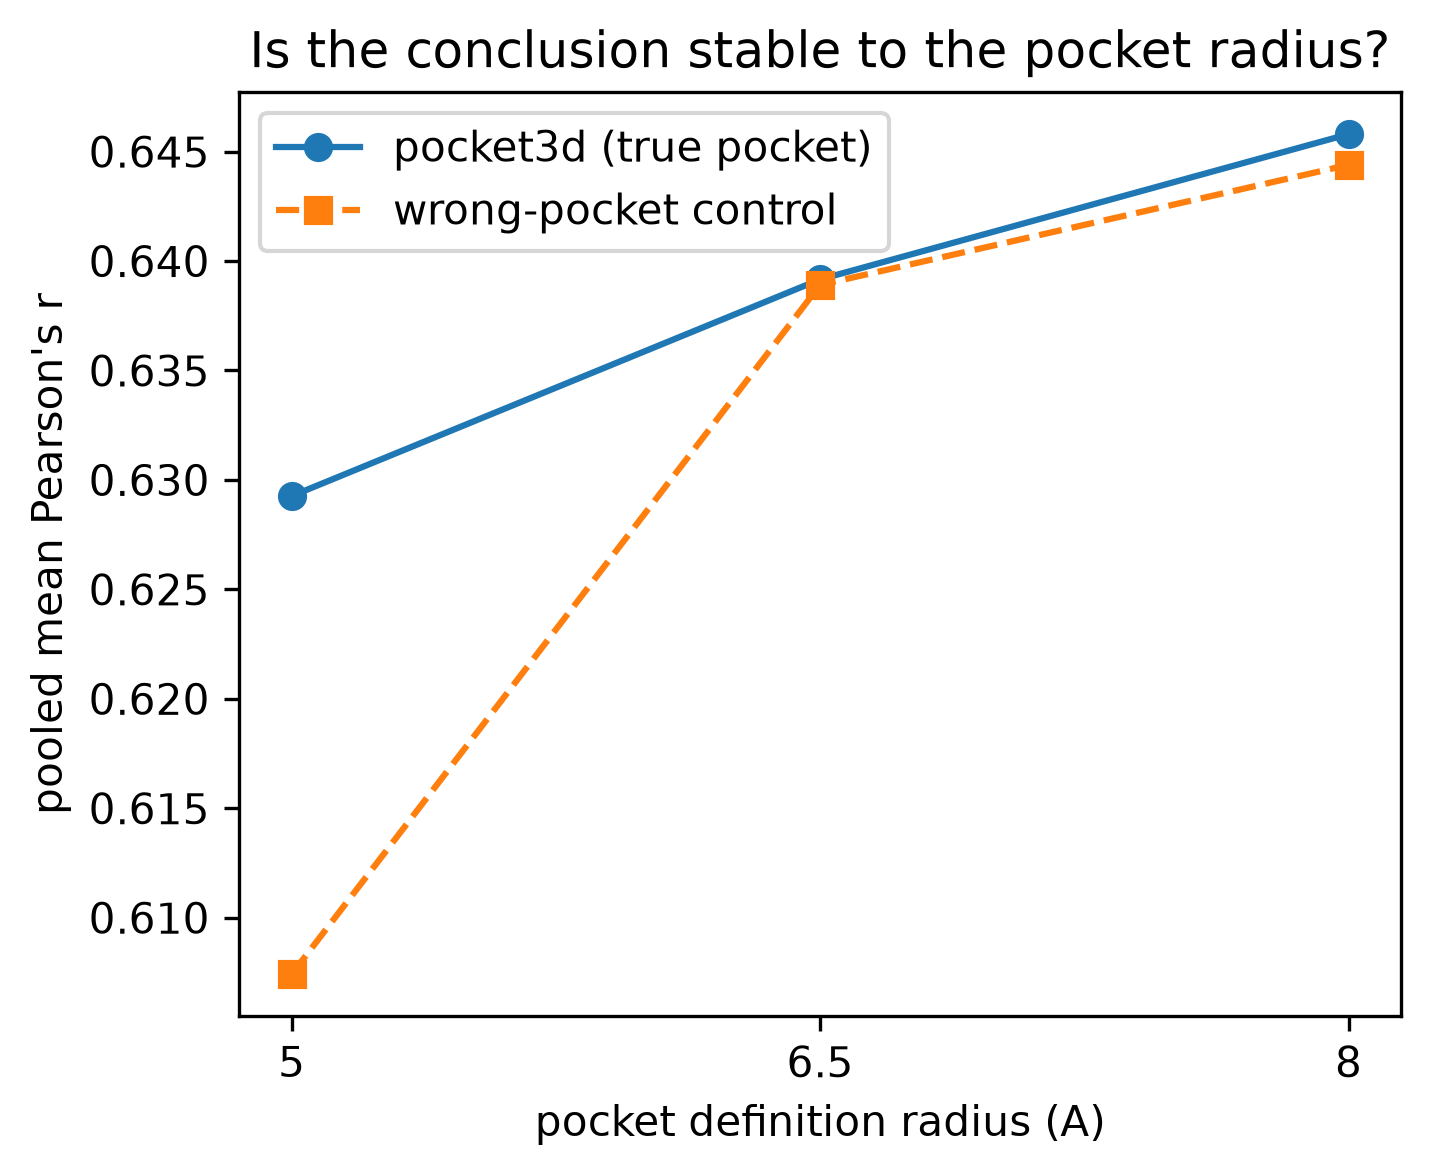
\includegraphics[width=0.85\textwidth]{../figures/fig_radius_sweep.png}
\caption{Pocket-radius sweep (5.0/6.5/8.0\,\AA): pooled C$-$E difference
in Pearson $r$ per radius. No radius yields a significant advantage for
true-pocket geometry.}
\label{fig:radius}
\end{figure}

\subsection{Variance decomposition}

Across the 280 measured E3 cells, receptor identity explains 84.5\% of
outcome variance, model arm 2.7\%, and residual (seed$\times$receptor)
12.8\%; mean within-cell seed sd is 0.028. The split-protocol effect
(E3$-$E5, mean $+0.255$) is two orders of magnitude larger than every
arm effect. The practical message for practitioners: choosing the
receptor family and the evaluation protocol matters ~30$\times$ more
than choosing among these conditioning architectures.

\subsection{Mutation probe: honestly not run}

The pre-registered mutation probe (do point mutations with measured
affinity shifts let 3D grounding respond where 1D cannot?) requires
mutant-specific records in the frozen artefacts. The frozen ChEMBL
export carries no \texttt{assay\_description} column, so mutant records
cannot be identified without re-downloading --- forbidden by the
frozen-data rule. The probe is recorded as \textbf{not run} with the
reason attached (\texttt{mutation\_probe.json}); no substitute,
simulation, or estimate was fabricated.

\section{Discussion}

The combined evidence from Paper~1 and this study now localises the
bottleneck precisely. Ligand fingerprints carry essentially all of the
learnable affinity signal in this regime; receptor conditioning --- 1D or
3D, faithful or deliberately corrupted --- moves performance by at most
hundredths of a Pearson $r$, and corrupted conditioning is
indistinguishable from faithful conditioning. The failure is not in the
geometry pipeline (crystal and AFDB geometry agree to $\Delta r\le
0.016$), not in the pocket definition (stable across 5.0--8.0\,\AA), and
not in statistical power (45 paired samples per comparison, CIs of
$\pm 0.02$).

Three explanations are consistent with the measurements, and we do not
adjudicate among them: (i) ESM-2 residue embeddings already saturate
whatever pocket-identity information the small conditioning heads can
use, so explicit geometry adds nothing they lack; (ii) affinity in this
data regime is dominated by ligand properties, with receptor identity
acting mostly as a per-receptor intercept that a shared model already
captures; (iii) the conditioning heads are too small to exploit
geometric detail. What the measurements \emph{do} rule out is the claim
that current protein foundation model representations, conditioned
through small heads, extract usable pocket-geometry signal for
cross-family affinity prediction on ChEMBL-scale data.

\paragraph{Limitations.} The study covers eleven receptors from two
families (aminergic GPCRs, one ion channel) and one ligand featurisation
(Morgan fingerprints); results may not transfer to structure-exclusive
ligand series or to end-to-end 3D models trained at scale. The
conditioning heads are deliberately small; a much larger 3D model might
behave differently, though at the cost of the controlled comparison this
study is designed to provide. The mutation probe was not run (no
mutant-identifying fields in the frozen artefacts).

\section{Conclusion}

On 41{,}271 measured ChEMBL pairs, eleven receptors, six pre-registered
model arms, and two evaluation protocols, explicit 3D pocket geometry
--- from crystals or from AlphaFold --- does not beat its own controls.
The wrong-pocket control, transplanted from 1D conditioning to full 3D
message passing, still reproduces the 3D arm's performance. This is a
decisive negative result with a practical positive: the field's
1D-versus-3D question, for foundation model representations at current
quality, has a measured answer --- and the answer is that pocket
geometry is not yet the binding constraint. We release every artefact
needed to check, extend, or overturn this conclusion.

\section*{Data and Software Availability}
No new bioactivity data were generated; all 41{,}271 pairs derive from
ChEMBL and were frozen in the companion study. All software required to
reproduce every figure and table --- the complete Python pipeline,
environment specification, automated test suite, and frozen
machine-readable artefacts (CSV/JSON/NPZ with SHA-256 checksums) --- is
publicly available at \url{https://github.com/MD-Mushfiqur123/MEG-BAR}
(\texttt{paper2/} tree). This preprint is archived at
\url{https://doi.org/10.6084/m9.figshare.35010655}; the companion
preprint (Paper~1) is archived at
\url{https://doi.org/10.6084/m9.figshare.35002837}.

\appendix
\section{Reproducibility}

\textbf{Environment.} Python 3.12, PyTorch (CPU), NumPy, SciPy,
matplotlib; exact versions in \texttt{paper2/ENVIRONMENT.md}. All runs
CPU-only (no GPU); total measured training time 2.34\,h across 280
models.

\textbf{One-command reproduction.} From the repository root:
\begin{verbatim}
make paper2-stage1   # structures, pockets, mapping, manifest
make paper2-stage2   # distances, contacts, graphs, geometry
make paper2-stage3   # six arms, scaffold-disjoint, resume store
make paper2-stage4   # master table, temporal, statistics, budget
make paper2-stage5   # crystal-vs-AF, radius sweep, verdicts
make paper2-test     # 55 artefact tests
\end{verbatim}
Every stage is checkpointed; re-running skips completed phases and
regenerates figures from frozen stores.

\textbf{Artefact integrity.} \texttt{paper2/data/structures/manifest.json}
records SHA-256 for every structure and feature file; the result stores
(\texttt{stage3/arms\_scaffold\_results.json},
\texttt{stage4/temporal\_results.json}, \texttt{stage5/*.json}) record
per-seed metrics, hyperparameters, and skip reasons for every run.

\section{Defect register (summary)}

Two defects were catalogued and fixed during Stages 4--5, per the
non-negotiable that failed claims are recorded, never quietly dropped:
(5) the first H4 operationalisation (sign-agreement on noise-level
differences) was invalid and was replaced by the pre-registered
verdict-transfer test --- both versions are retained in the register;
(6) a radius-sweep filename/prefix mismatch between Phase 28 and the
Stage 6 generators was fixed before publication; no measured number
changed. The full register, including Stages 1--3 defects (anchor
corrections, the Arm F context-dispatch bug, AFDB version drift), is in
\texttt{paper2/DEFECT\_REGISTER.md}.

\end{document}
